\NeedsTeXFormat{LaTeX2e}

% The following saves the original definitions of \geq and \leq (guide only).
\let\realgeq\geq
\let\realleq\leq

\documentclass{fac}

\ifprodtf \else \usepackage{latexsym}\fi

% The following macros automatically define symbols to be used in Table 1 of
% the authors' guide, using characters from the AMS symbol font MSAM.

\newcommand\black{\ensuremath{\blacktriangleright}}
\newcommand\white{\ensuremath{\vartriangleright}}

\newif\ifamsfontsloaded
\ifprodtf
  \newcommand\whbl{\white\kern-.1em--\kern-.1em\black}
  \newcommand\blwh{\black\kern-.1em--\kern-.1em\white}
  \newcommand\blbl{\black\kern-.1em--\kern-.1em\black}
  \newcommand\whwh{\white\kern-.1em--\kern-.1em\white}
  \amsfontsloadedtrue
\else
  \checkfont{msam10}
  \iffontfound
    \IfFileExists{amssymb.sty}
      {\usepackage{amssymb}\amsfontsloadedtrue
       \newcommand\whbl{\white\kern-.125em--\kern-.125em\black}%
       \newcommand\blwh{\black\kern-.125em--\kern-.125em\white}%
       \newcommand\blbl{\black\kern-.125em--\kern-.125em\black}%
       \newcommand\whwh{\white\kern-.125em--\kern-.125em\white}}
      {}
  \fi
\fi

%% Macros for the guide only %%
\newcommand\eg{\textit{e.g.\ }}
\newcommand\etc{\textit{etc}}
\newcommand\hatp{\skew3\hat{p}}
\newcommand\lra{\ensuremath{\quad\longrightarrow\quad}}
\providecommand\AMSLaTeX{AMS\,\LaTeX}
%% End of macros for the guide %%

\newtheorem{theorem}{Theorem}[section]

\title{A Relational Static Semantics for\\
		\ Call Graph Construction}

\author[Xilong Zhuo and Chenyi Zhang]
    {Xilong Zhuo$^1$ and Chenyi Zhang$^2$\\
     $^1$College of Information Science and Technology, Jinan University, China\\
     $^2$College of Information Science and Technology, Jinan University, China}

\correspond{Chenyi Zhang.
            e-mail: chenyi\_zhang@jnu.edu.cn}

%\pubyear{2000}
\pagerange{\pageref{firstpage}--\pageref{lastpage}}

\newcommand{\less}{\sqsubseteq}
\newcommand{\tflow}{\dashrightarrow}
\newcommand{\hflow}{\longrightarrow}
\newcommand{\lhflow}[1]{\stackrel{#1}{\hflow}}

\usepackage{graphicx}
\usepackage{color}
\definecolor{lbcolor}{rgb}{1,1,1}

\usepackage{listings}
\lstset{
  backgroundcolor=\color{lbcolor},
  language=java,
  frame=single,
  numbers=left,
  stepnumber=1,    
  firstnumber=1,
  numberfirstline=true,
  captionpos=b,
  keywordstyle=\color[rgb]{0,0,1},
  commentstyle=\color[rgb]{0.133,0.545,0.133},
  stringstyle=\color[rgb]{0.627,0.126,0.941}
}

\usepackage{amsfonts}

\begin{document}
\label{firstpage}

\makecorrespond

\maketitle

\begin{abstract}
The problem of resolving virtual method and interface calls in object-oriented languages has been a long standing challenge to the program analysis community. The complexities are due to various reasons, such as increased levels of class inheritance and polymorphism in large programs. In this paper, we propose a new approach called type flow analysis that represent propagation of type information between program variables by a group of relations without the help of a heap abstraction. We prove that regarding the precision on reachability of class information to a variable, our method produces results equivalent to that one can derive from a points-to analysis. Moreover, in practice, our method consumes lower time and space usage, as supported by the experimental results.
\end{abstract}

\begin{keywords}
Type Analysis; Static Analysis; Method Resolving; Call Graph
\end{keywords}

\section{Introduction}\label{sec:introduction}

For object-oriented programming languages, virtual methods (or functions) are those declared in a base class but are meant to be overridden in different child classes. Statically determine a set of methods that may be invoked at a call site is important to program optimization...
\section{Type Flow Analysis}\label{sec:type-flow-analysis}
We define a core calculus consisting of most of the key object-oriented language features...
\subsection{c$\tflow$ y}
\subsection{x$\less$ y}
\subsection{x$\lhflow{f}$ y}

\section{Implementation}\label{sec:implementation}
The analysis algorithm is written in Java, and is implemented in the Soot framework, the most popular static analysis framework for Java. We use jimple as our intermediate representation. 
We do not take common types (\eg, int and float) under our consideration. That are irrelevant to our analysis. We keep method invocation from Java advanced features liked reflection or JNI as unresolvable. More detail will be discussed in \ref{subsubsec:reflection-call} and \ref{subsubsec:jni-call}. Conservative approximation is performed on invocation of methods from libraries (\eg, JDK) and array accesses. We will describe these strategies in \ref{subsubsec:library} and \ref{subsubsec:array-approximation}.

A Static analysis tool is implemented to process our algorithm and extract static result of type solution. In addition, we implement a dynamic profiler to record the run time type of variable, which can be used to compare with the static result. Detail of static analysis tool and dynamic profiler will be discuss in ~\ref{subsec:static-analysis-tool} and ~\ref{subsec:dynamic-profiler}, respectively.

\subsection{Static Analysis Tool}\label{subsec:static-analysis-tool}
Our static analysis tool is implemented in Java and aims to analyze Java programs. It takes Java bytecode files as input. Any other format of Java code will be accepted if it can be translated to jimple representation by Soot(\eg, jar files). The implementation of our static analysis tool can be splited into four step as follow.
\begin{itemize}
\item Code translation\\
Target code is loaded by Soot and translated to IR of jimple format.
\item Basic relation generation\\
We iterate all statements on jimple IR to generate those basic relations based on the basic relation difinition. 
\item Fixpoint calculation\\
After basic relations are generated, we use the extended relation rule to perform fixpoint calculation.
\item Result extraction\\
When the fixpoint is achieved, all set of reaching types of all variable are immutable. We extract those set of reaching types as our final result.
\end{itemize}
Fig~\ref{fig:static-process} shows the whole process of our static analysis tool. Data input and generated are represented in dash arrow. The final result is generated in the ``Result Extraction'' phase and represented in green background.

\begin{figure}
\centering
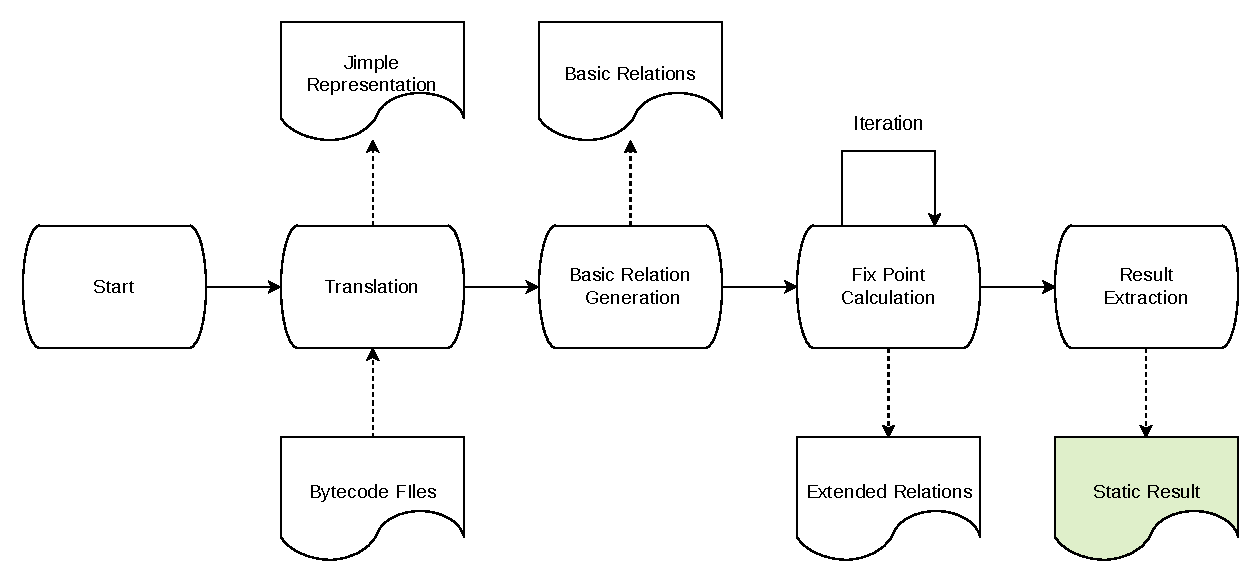
\includegraphics[width=16cm,height=6cm]{static-process.pdf}
\caption{Process of static analysis tool}
\label{fig:static-process}
\end{figure}

\subsection{Dynamic Profiler}\label{subsec:dynamic-profiler}
Since the benchmarks do not provide the grountruth of run-time type of method receiver, we implement a dynamic profiling tool to record  types which a receiver can access at run-time. To achieve this, we instrument statements into the target benchmark. After this instrumentation, the run-time type will be extracted during the benchmark execution. We consider this output as groundtruth and compare it with our static result in section ~\ref{subsec:precision}. There are four manners to instrument the source code to record the run-time type of a method receiver.
\begin{itemize}
\item Insert First\\
In this manner, the type-recorded statements will be insert before the first statement of a method block and the type of ``this'' reference in that method will be recorded. The reason we only have to record ``this'' reference is that a receiver is always passed into ``this'' reference in a method, except for static methods. 
\item Insert Before\\
Statements will be inserted before invocations and the type of receiver will be recorded in this manner. It is more straightforward than the method we discuss about recording ``this'' reference.
\item Insert Last\\
This manner is similar with ``Insert First'', except that statements are inserted after the last statement of a method block. We also record ``this'' reference in this way.
\item Insert After\\
Statments will be inserted right after invocations and the type of receiver will be recorded. It is similar with ``Insert Before'', except that statements are inserted at different position. We take this manner in our implementation and the reason will be discuss in section ~\ref{subsubsec:instrument}
\end{itemize}
%\subsubsection{Insert First}\label{subsubsec:insert-first}
%In this manner, the type-recorded statements will be insert before the first statement of a method block and the type of ``this'' reference in that method will be recorded. The reason we only have to record ``this'' reference is that a receiver is always passed into ``this'' reference in a method, except for static methods. 
%\subsubsection{Insert Before}\label{subsubsec:insert-before}
%Statements will be inserted before invocations and the type of receiver will be recorded in this manner. It is more straightforward than the method we discuss about recording ``this'' reference.
%\subsubsection{Insert Last}\label{subsubsec:insert-last}
%This manner is similar with ``Insert First'', except that statements are inserted after the last statement of a method block. We also record ``this'' reference in this way.
%\subsubsection{Insert After}\label{subsubsec:insert-after}
%Statments will be inserted right after invocations and the type of receiver will be recorded. It is similar with ``Insert Before'', except that statements are inserted at different position. We take this manner in our implementation and the reason will be discuss in section ~\ref{subsubsec:instrument}
\subsubsection{Our Instrumentation Manner}\label{subsubsec:instrument}
We take ``Insert After'' as our instrumentation manner. The reason is mainly due to the Java specification of constructor that the first statement in constructor should be either another constructor of its own or its super class. Therefore, we will get JVM voilation error if we instrument a statement before the first statement in construtor. We illustrate this example on Listing~\ref{lst:spec-constructor}. So both ``Insert First'' and ``Insert Before'' manners can not be applied under this circumstance. We choose ``Insert After'' over ``Insert Last'' for reason that it's more straightforward. The code before and after instrumentation are shown in Listing~\ref{lst:before-instru} and Listing~\ref{lst:after-instru}, respectively. For Listing~\ref{lst:after-instru}, at line 5, the funtion $RecordUtils.id()$ takes an invocation expression ($invokeExprssion$) and a method receiver ($b$) as parameters and return an unique representation string for this invocation. For this example, the unique representation is ``A:m1:b:B:m2:4''. This means $b$ will call method $m2$ of class $B$, at line 4 in method $m1$ of class $A$. It also shows that $b$ is of type $B$ at this position.

\begin{lstlisting}[caption={Java specification on constructor},label={lst:spec-constructor}]
class A {
  public A() {
    //insert statements here will violate JVM specification
    super();	//invoke super class constructor
  }
  public A(int i) {
    //insert statements here will violate JVM specification
    this();    //inovke another constructor of its own
  }
}
\end{lstlisting}

\begin{lstlisting}[caption={Example code before instrumentation},label={lst:before-instru}]
class A {
  public void m1() {
    B b = new B();
    b.m2();    //invocation here
  }
}
\end{lstlisting}

\begin{lstlisting}[caption={Example code after instrumentation},label={lst:after-instru}]
class A {
  public void m1() {
    B b = new B();
    b.m2();    //invocation here
    String record = RecordUtils.id(invokeExpression, b);
    RecordUtils.record(record);
  }
}
\end{lstlisting}

\section{Evaluation}\label{sec:evaluation}
We evaluate our approach by measuring its performance on SPECjvm2008, which contains $12$ benchmark programs in total. We conduct all of our experiments on a laptop equipped with an Intel i5-8250U CPU at 1.60 GHz and 8 GB memory, running Ubuntu 16.04LTS with OpenJDK 1.8.0.

We compare our approach against the default implementation of Class Hierarchy Analysis (CHA) and context-insensitive points-to analysis that are implemented by Soot team. The reason we do not compare against Variable Type Analysis (VTA) due to its unavaliable implementation. The only implementation for Java we can find is also implemented by Soot team, but it is embeded as a subprocess to optimize points-to analysis. Under this circumstance, we compare our approach against VTA in precision with manual analysis in section~\ref{sec:introduction}. Implementation of VTA will be left for our future work. During the evaluation the following tow research questions are addressed.
\begin{itemize}
\item \textbf{RQ1} How efficient is our approach compared with the traditional class hierarchy analysis and points-to analysis?
\item \textbf{RQ2} How accurate is our type resolution when comparing with the other analysis?
\end{itemize}
We answer RQ1 and RQ2 in section~\ref{subsec:efficiency} and section~\ref{subsec:precision}, respetively.

\subsection{Efficiency}\label{subsec:efficiency}
We executed each benchmark program $10$ times with the CHA, PTA and TFA algorithms. We calculated the average time consumption...

\begin{figure}\centering
%\begin{table}[!htbp]\centering
\begin{tabular}{lcccccc}
	\hline
	\textbf{Benchmark} & \hspace{5pt}\textbf{T$_{\textsf{TFA}}(s)$} & \hspace{5pt}\textbf{R${\tflow}$}\hspace{5pt} & \hspace{5pt}\textbf{R$_{\less}$}\hspace{5pt} & \hspace{5pt}\textbf{R${\rightarrow}$} &\hspace{5pt}\textbf{R$_{total}$}\hspace{2pt}\\
	\hline
check & 10.46 & 6847 & 15599 & 10089 & 32535\\
compiler & 11.48 & 6665 & 14898 & 10433 & 31996\\
compress & 12.19 & 6410 & 14344 & 10322 & 31076\\
crypto & 9.21 & 6459 & 14424 & 10152 & 31035\\
derby & 11.65 & 6887 & 14853 & 10603 & 32343\\
helloworld & 13.10 & 6149 & 13652 & 10071 & 29872\\
mpegaudio & 10.65 & 6197 & 13737 & 10084 & 30018\\
scimark & 11.24 & 6366 & 14678 & 10214 & 31258\\
serial & 10.98 & 6627 & 14309 & 10341 & 31277\\
startup & 10.73 & 6239 & 13723 & 10094 & 30056\\
sunflow & 11.12 & 6167 & 13675 & 10077 & 29919\\
xml & 13.84 & 6866 & 16039 & 11060 & 33965\\
	\hline
\end{tabular}
\caption{Runtime cost with different analysis}
\label{experiment:TimeCost}
%\end{table}
\end{figure}

\subsection{Precision}\label{subsec:precision}
\subsubsection{Reflection Call}\label{subsubsec:reflection-call}
Reflection in Java programming language is a advanced feature which provides ability to inspect and manipulate a Java class at runtime. It brings in extra complexity on programs and the behaviour is hard to predict statically. In Listing~\ref{lst:reflection} we pick some codes using reflection in the benchmark programs to discuss how reflection works and what is our treatment on that. Note that we reorganize and simplify the real code a little to concentrate on the main point of reflection usage. We discuss in three cases:
\begin{itemize}
\item Object Creation \\
Related codes range from line 6 to 10. A new obejct of type ``SPECJVMBenchmarkBase'' will be created by invoking the method ``$newInstance()$'' on variable $c$ at line 10. $c$ is an object of ``Constructor'' type and it refers to a specific constructor of class ``SPECJVMBenchmarkBase''. Our method discard the type information of new object in these case because it's difficult to statically identify which constructor will be invoked. \eg, At line 6, If statement $Class.forName()$ receive argument from outside liked user input or loading file with content of class name, then we could not find out the real type of $benchmarkClass$. As a result, the run time type of $c$ and $benchmark$ could not be identified neither.
\item Method Invocation\\
After a new object is instantiated, we can get an object of ``Method'' type, referring to a specific method of a class, and call the method named ``invoke()'' of that object. This effect is just like a normal invocation at line 12. The invocation receiver is passed to the first argument of method ``invoke()''. If this invocation is static, a \textbf{null} reference will be passed to the first argument. We do not consider these effects of method invocation in reflection manner for the same reason we discuss about object creation.
\item Field Modification\\
The way to change a field using reflection is similar to processing method invocation. The last two line illustrate changing value of a field named ``f'' on object ``benchmark'' into a new object. We discard this effect as well because of the difficulty on analyzing which class holds the target field.
\end{itemize}

\begin{lstlisting}[caption={Example code of reflection},label={lst:reflection}]
public static void runSimple(Class benchmarkClass, String [] args) {
  ...
  ...
  Class[] cArgs = { BenchmarkResult.class, int.class };
  Object[] inArgs = { bmResult, Integer.valueOf(1)};
  Class benchmarkClass = Class.forName("spec.harness.SpecJVMBenchmarkBase");
  Constructor c = benchmarkClass.getConstructor(cArgs);

  // Object creation using reflection
  SpecJVMBenchmarkBase benchmark = (SpecJVMBenchmarkBase)c.newInstance(inArgs);
  // normal method invocation
  benchmark.harnessMain();
  
  // method invocation
  Method harnessMain = benchmarkClass.getMethod("harnessMain", new Class[]{});
  // just like line 11 but in reflection manner
  harnessMain.invoke(benchmark, new Object[]{}); 
  
  Method setup = benchmarkClass.getMethod( "setupBenchmark", new Class[]{});
  // static invocation
  setup.invoke(null, new Object[]{});
  
  // field modification
  Field f = benchmarkClass.getField("f");
  f.set(benchmark, new Object());
}
\end{lstlisting}

\subsubsection{Java Native Interface Call}\label{subsubsec:jni-call}
Java Native Interface (JNI) is a standard Java programming interface which provide ability for Java code to interoperate with application or library written in other programming languages, such as C, C++ or assembly. We show the usage of JNI in Listing~\ref{lst:jni}. Method ``$m()$'' is defined as a native method and should not be implemented in Java. This program will load a native library named ``$lib$'', in which the method ``$m()$'' is actually implemented in different program languages. We do not consider JNI calls in our algorithm since the code is not written in Java. Analyzing that code and the communication between Java and other languages are out of our research scope. As a consequence, the effect of that invocation ``$a.m()$'' at line 8 will be discarded.

\begin{lstlisting}[caption={Example code of JNI},label={lst:jni}]
public class A {
  public native void m();
  static {
    System.loadLibrary("lib");
  }
  public static void main(String[] args) {
    A a = new A();
    a.m(); <---
  }
}
\end{lstlisting}

\subsubsection{Library}\label{subsubsec:library}
Library are those codes included in the application and used to accomplish specific function(\eg, JDK library, three-party library). Listing~\ref{lst:jdk} shows a common case of JDK invocation. We do not analyze the detail logic inside library code which are written at line 10-11. Instead, we perform an over approximation on library invocation, based on the method difinition which appears at line 9. We assume that library invocation will return the difinition type and any subtype of this difinition type as the result type. For Listing~\ref{lst:jdk}, $sb2$ will receive $\{StringBuilder,\ any\_subtype\_of\_StringBuilder\}$ as the set of reaching types under this over approximation strategy.

\begin{lstlisting}[caption={Example of JDK library call},label={lst:jdk}]
import java.lang.StringBuilder;

public void m() {
  StringBuilder sb = new StringBuilder();
  StringBuilder sb2 = sb.append("abc"); <---
}

//  @Override
//  public StringBuilder append(String str) {
//    ...
//    ...
//  }
\end{lstlisting}

\subsubsection{Array Approximation}\label{subsubsec:array-approximation}
We perform a conservative treatment on array accesses that all type information that flows to one member of an array flows to all members of that array. Codes in Listing~\ref{lst:array} are used to explain how this approximation works. Type information of $A$ and $B$ are flow to the first member and the second member of array $arr$, respectively. We approximate that these two type information flow to array $arr$. Loadding an element of array will receive all types that array can access(\eg, $b$ will receive $\{A, B\}$ as the set of reaching types, which is the same set of types that array $arr$ can access).

\begin{lstlisting}[caption={Example of array access},label={lst:array}]
public void m() {
  Object[] arr = new Object[2]{};
  arr[1] = new A();
  arr[2] = new B();
  Object b = arr[1];  <---
}
\end{lstlisting}

\section{Related Work}\label{sec:related-work}
There are not many works focusing on general purpose call graph construction algorithms, and we give a brief review of these works first.

\section{Conclusion}\label{sec:conclusion}
In this paper we have proposed Type Flow Analysis (TFA), an algorithm that constructs call graph edges for Object-Oriented programming languages.

\label{lastpage}

\end{document}
